\section{Implementierung}
\label{cha:implementierung}

Die Implementierung dieser Applikation erfolgte wie gefordert in \textsl{C++}. Es handelt sich hierbei nicht nur um die Implementierung des bereits 
beschriebenen Synchronisationsalgorithmus. Es musste auch die Netzwerkkommunikation zwischen den Programmen und die interne Kommunikation zwischen den 
einzelnen Komponenten der Applikation realisiert werden.

\subsection{Synchronisationsablauf}
\label{sec:sychronisierung}

Der Verlauf eines Synchronisationsprozesses zwischen einem Synchronisations-Client und einem Synchronisations-Server sieht wie folgt aus:
\begin{enumerate}
\item Der Client initialisiert die Kommunikation, indem er eine Anfrage an den Server schickt, ihm eine Liste sämtlicher seiner synchronisierbaren 
      Dateien zu schicken.
\item Der Server geht dieser Anfrage nach und schickt dem Client ein Liste sämtlicher Dateien.
\item Der Client vergleicht nun diese Liste mit seinen lokalen Dateien. Dateien, die er nicht kennt, werden vom Server angefordert, Dateien, 
      von denen er weiß, dass sie bei ihm bereits gelöscht sind, werden dem Server entsprechend als \emph{zu löschen} vermittelt. Bei Lokale Dateien, 
      die nicht in der List des Servers aufscheinen, schickt der Client eine Anfrage, ob diese gelöscht wurden oder der Server sie vom Client braucht.  
      Alle restlich Dateien, die, die mit ihrem Namen bzw. Pfad sowohl beim Client als auch beim Server vorhanden sind, werden auf Übereinstimmung bezüglich 
      Zeitstempel und Gesamtsignatur überprüft. Für die Dateipaare, bei denen diese Werte unterschiedlich sind, wird der Synchronisationsalgorithmus 
      initialisiert und der Client schickt eine entsprechende Synchronisationsanfrage mit den schwachen Signaturen an den Server.
\item Der Server folgt den Nachrichten des Clients und sendet entsprechende Antworten zurück (z.B. eine angeforderte Datei). 
      Bekommt der Server eine Synchronisationsanfrage so überprüft er die schwachen Signaturen mit der seiner lokalen Datei. Gibt es Übereinstimmungen, 
      so schickt der Server ein Anfrage für die starken Signaturen der übereinstimmenden Blöcke an den Client. Abhängig von den Zeitstempeln der Dateien 
      schickt der Server für die nicht übereinstimmenden Blöcke entweder seine Inhalte an den Client oder fragt die entsprechenden Inhalte beim Client an. 
      (Der mit dem kleineren Zeitstempel, sprich der älteren Datei, muss sich die Daten holen, um den neueren Stand der Datei rekonstruieren zu können.)
\item Der Client schickt die geforderten starken Signaturen an den Server und, wenn gefordert, auch den Inhalt der nicht übereinstimmenden Blöcke bzw. 
      speichert die erhaltenen Korrekturdaten zur späteren Dateikonstruktion.
\item Der Server überprüft die starken Signaturen des Clients mit seinen eigenen. Wie bei den schwachen auch, schickt er für die nicht übereinstimmenden 
      Blöcke die Korrekturdaten an den Client bzw. fordert sie an. Mit den übereinstimmenden Blöcken wird nichts mehr gemacht.
\item Der jenige, der die Korrekturdaten erhalten hat, (Client oder Server) muss nun die neue Datei rekonstruieren. Dafür wird aus Sicherheitsgründen eine 
      temporäre Datei im Unterverzeichnis \textit{.sync} erstellt. Diese wird nun in der entsprechenden Reihenfolge nacheinander mit den Korrekturdaten 
      befüllt. Für die Stellen, für die es keine Korrekturdaten gibt, wird der Inhalt aus der alten, lokalen Datei verwendet, da diese an dieser Stelle gleich 
      mit der neueren sein muss, zumindest laut den Signaturen, sonst gebe es ja Korrekturdaten dafür. Am Ende wird die zusammengebaute Datei an ihren 
      richtigen Ort verschoben und die alte somit überschrieben.
\end{enumerate}

Ein bedeutender Unterschied zum in Abschnitt \ref{sec:rsync} beschriebenen Algorithmus von \textit{rsync} ist, dass fast alle Entscheidungen vom Server
gefällt werden. Hingegen bei \textit{rsync} werden die Entscheidungen und so auch die Vergleiche der Signaturen auf die beiden beteiligten 
Netzwerkprozesse aufgeteilt. Diese Ausführung des Synchronisationsverlaufs hat weniger mit Restriktionen in der Verwirklichung als mit
einer strukturellen Entscheidung, dass der Server die Deutungshoheit haben sollte, zu tun. Wobei angemerkt werden muss, dass dies zu einer größeren
Anzahl an Nachrichten zwischen Client und Server führt.

\subsection{Netzwerkkommunikation}
\label{sec:netzwerkkom}

Die Netzwerkkommunikation ist mithilfe von \textit{Protocol Buffers}\cite{proto} für die Serialisierung der Nachrichten und \textit{Asio}\cite{asio} 
zur Übertragung der serialisierten Nachrichten realisiert. Da \textit{Asio} eine Bibliothek zur textbasierten Netzwerkübertragung ist und 
\textit{Protocol Buffers} die Nachrichten in ein binäres Format serialisiert, kann es dazu kommen, dass in den Nachrichten das Zeichen zur Trennung 
von Nachrichten und dem Beenden des Leseflusses für \textit{Asio} vorkommt. In diesem Fall ist es das \textit{Newline}-Zeichen, \verb|\n|. 
Da \textit{Protocol Buffers} dieses Zeichen im Serialisierungsformat durchaus benutzt und theoretisch jeder beliebige Wert für ein Byte in 
seiner serialisierten Nachricht vorkommen kann, kann weder \verb|\n| noch ein anderes Zeichen als Trennzeichen benutzt werden.
Daher werden die serialisierten Nachrichten noch zusätzlich in Base 64 kodiert und, da die Menge der 64 Zeichen von Base 64 das Newline-Zeichen 
nicht enthält, kann dieses ohne Probleme als Trennzeichen benutzt werden. Da die Nachrichten an einem Ende kodiert werden müssen sie dementsprechend 
auch am anderen Ende wieder dekodiert werden, noch bevor sie deserialisiert werden können. Die Base 64-Kodierung stellt kein besondere Leistungshinderung
dar, vergrößert die zu transferierenden Daten aber doch um immerhin ein Drittel. Allerdings ist Base 64 nun Mahl wichtig für die funktionsfähige
Interoperation der binären Serialisierung und der textbasierten Netzwerkübertragung.

\subsection{Interne Kommunikation}
\label{sec:internekom}

Die Applikation besteht aus mehreren Prozessen, die voneinander halbwegs unabhängig agieren sollten. Es sind drei Haupt-Prozesse, 
die für die Funktionstüchtigkeit der Applikation verantwortlich sind:
\begin{itemize}
\item Der \textbf{Server} ist für die Kommunikation mit anderen Clients zuständig und startet für jede Verbindung einen eigenen Thread.
\item Der \textbf{Client} ist für die Kommunikation mit einem Server zuständig.
\item Der \textbf{File Operator} ist für den gesamten Synchronisationsablauf und der Kommunikation mit dem Dateisystem zuständig, 
      sowohl Client- als auch Server-seitig, und kann aus mehreren Threads bestehen. 
\end{itemize}

Neben diesen drei Hauptprozessen gibt es noch einen Prozess, welcher sich um die \textbf{Kommandozeile} kümmert. 

\subsubsection{Pipe Interfaces}
\label{sec:pipe}

Die Kommunikation zwischen diesen Akteuren erfolgt über Pipes. Der File Operator bekommt das empfangende Ende einer Pipe und der Server und der Client 
(auch die Kommandozeile) bekommen das sendende Ende dieser Pipe, über welches sie Anfragen an den File Operator schicken können, welche dieser bearbeiten 
soll. Damit der File Operator ihnen Antworten auf ihre Anfragen zurückschicken kann, schicken sie das sendende Ende einer Pipe, welche sich in ihrem Besitz 
befindet, mit. Dieses kann der File Operator benutzen, um ihnen Rückmeldungen zu schicken.

Um die Unterscheidung von sendenden und empfangenden Enden von Pipes zu ermöglichen, werden Interfaces (rein abstrakte Klassen) und Klassenvererbung 
benutzt. Bei den sendenden und empfangenden Enden einer Pipe handelt sich um zwei Interfaces, welche von der Pipe implementiert werden.

\begin{figure}
    \centering
    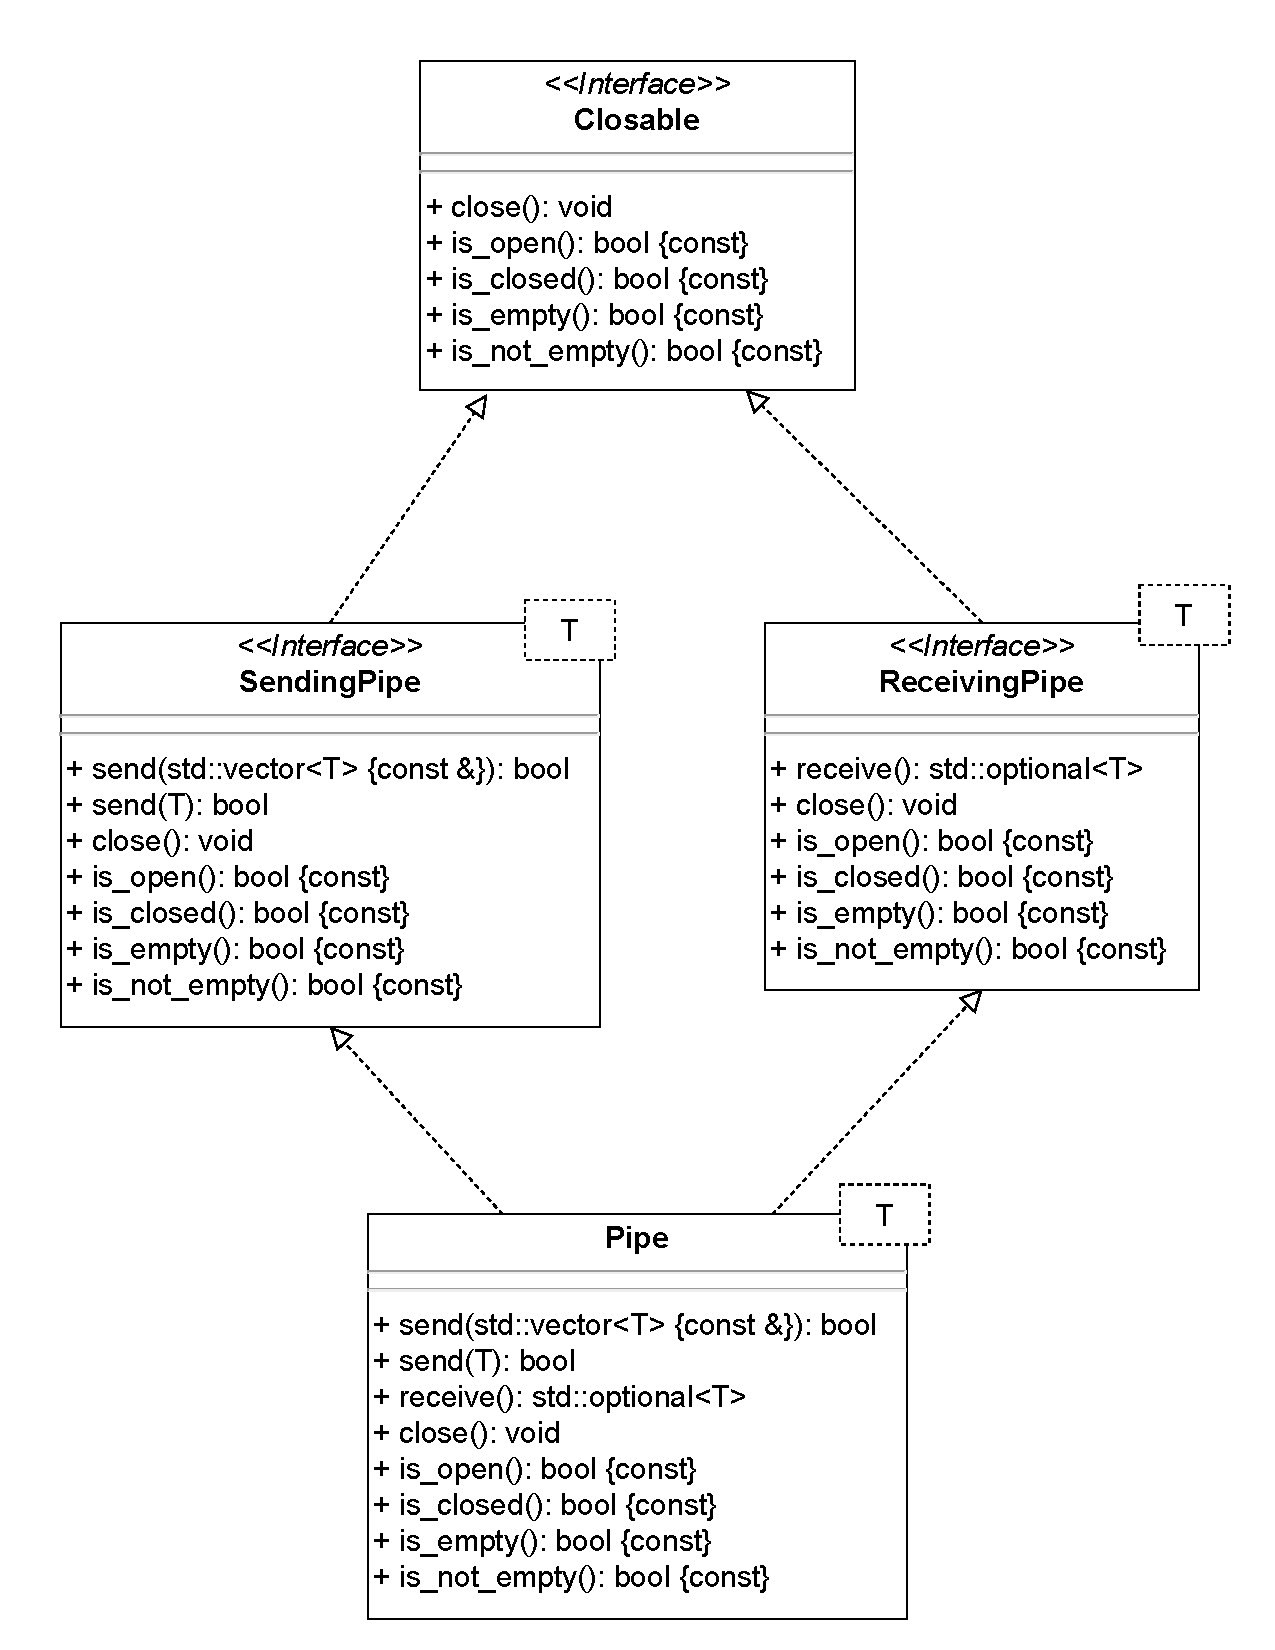
\includegraphics[width=\textwidth]{images/pipe_uml.pdf}
    \caption{UML-Klassendiagramm von Pipe}
    \label{fig:uml}
\end{figure}

Wie aus dem Klassendiagramm in Abbildung \ref{fig:uml} ersichtlich ist, haben das sendende Ende, \verb|SendingPipe|, und das empfangende Ende, 
\verb|ReceivingPipe|, eine Menge aus gemeinsamen Operationen, welche im Interface \verb|Closable| definiert sind, ein Pipe ist nämlich schließbar. 
Was aus dem Diagramm auch noch ersichtlich ist, ist dass die beiden Enden der Pipe und so auch die Pipe im Ganzen generisch für einen beliebigen Typ $T$ sind. 
Soll ein Prozess mit einer Pipe jetzt nur senden bzw. nur empfangen können, so bekommt dieser nur die Schnittstelle \verb|SendingPipe| bzw. 
\verb|ReceivingPipe| zur Verfügung gestellt.

Nun folgt eine etwas genauere Betrachtung der Implementierung von \verb|Pipe|, da diese schließlich auch Thread-sicher sein muss.

\subsubsection{Senden -- Pipe::send}
\label{sec:send}

\noindent\hrulefill\par
\begin{minipage}{\linewidth}
\begin{lstlisting}[language=C++, caption=Senden einer Nachricht ... bool send(T msg)]
std::lock_guard pipe_lck{pipe_mtx};
if (is_open()) {
    msgs.push(std::move(msg));
    receiving_finishable.notify_one();

    return true;
}
else {
    return false;
}  
\end{lstlisting}
\end{minipage}

Hier sehen wir als erste, die Funktion zum senden, \verb|bool send(T msg)|. Da es sich um eine schließbare Pipe handelt muss überprüft werden, 
ob die Pipe überhaupt noch offen ist. Von Interesse ist, dass das Mutex für die Pipe bereits vor der Überprüfung, ob die Pipe offen ist, also noch bevor 
überhaupt entschieden wurde, ob gesendet werden kann, gesperrt wird. Dies hat damit zu tun, dass die Funktion \verb|close()|, wie in Abschnitt \ref{sec:close}
gezeigt wird, zum Schließen der Pipe, auch dieses Mutex sperren muss. Durch das frühzeitige Sperren des Mutex beim Senden wird vermieden, dass die Pipe nach 
der Abfrage, ob sie offen ist, aber noch vor dem eigentlichen Senden, geschlossen wird. Das gleiche sieht man auch beim Empfangen in Abschnitt 
\ref{sec:receive}. Ansonsten passiert nicht viel mehr außer, dass die Nachricht eben in die Queue, welche der interne Speicher der Pipe ist, gelegt wird und 
anschließend wird ein Thread, welcher auf etwas Empfangbares wartet, benachrichtigt. Wenn das Senden erfolgreich war, sprich die Pipe offen war gibt es 
\verb|true| zurück, ansonsten \verb|false|. Neben dieser Methode gibt es noch \verb|bool send(std::vector<T>& msgs)|, zum Senden von mehreren Nachrichten. 
Diese funktioniert sehr ähnlich. Sie legt alle Nachrichten gleichzeitig in der erhaltenen Reihenfolge in die Queue, sobald dies möglich ist.

\subsubsection{Empfangen -- Pipe::receive}
\label{sec:receive}

\noindent\hrulefill\par
\begin{minipage}{\linewidth}
\begin{lstlisting}[language=C++, caption=Empfangen einer Nachricht ... std::optional<T> receive()]
std::unique_lock pipe_lck{pipe_mtx};
if (is_open()) {
    // warten, dass es etwas zum Empfangen gibt
    // oder die Pipe geschlossen wurde
    receiving_finishable.wait(
        pipe_lck, 
        [this](){ 
            return is_not_empty() || is_closed(); 
        }
    );

    if (is_open()) {
        T msg{std::move(msgs.front())};
        msgs.pop();

        return msg;
    }
    else {
        return std::nullopt;
    }
}
else {
    return std::nullopt;
}
\end{lstlisting}
\end{minipage}

Beim Empfangen mit \verb|std::optional<T> receive()| haben wir, wie bereits erwähnt, auch den Fall das als aller erstes die Mutex gesperrt wird und 
dann wird wieder überprüft, ob die Pipe offen ist. Ist die Pipe offen, wird mit der Condition Variable \verb|receiving_finishable| überprüft, 
ob es etwas zum Empfangen gibt und, falls nötig, darauf gewartet. Ist das Warten vollendet, wird nochmals überprüft, ob die Pipe offen ist, da das Warten 
auch durch das Schließen der Pipe beendet wird. Wenn ja, holt sich die Methode die vorderste Nachricht aus der Queue, löscht sie aus der Queue raus und 
gibt sie an den Aufrufer der Methode zurück. Konnte keine Nachricht geholt werden, da die Pipe geschlossen ist, wird Nulloption zurückgegeben. 
Mit einem optionalen Wert als Rückgabewert wird im Programm deutlich ausgedrückt, dass das Empfangen einer Nachricht nicht unbedingt erfolgreich sein muss.

\subsubsection{Schließen -- Pipe::close}
\label{sec:close}

\noindent\hrulefill\par
\begin{minipage}{\linewidth}
\begin{lstlisting}[language=C++, caption=Schließen der Pipe ... void close()]
std::lock_guard pipe_lck{pipe_mtx};
open = false;
receiving_finishable.notify_all();
\end{lstlisting}
\end{minipage}

Das Schließen der Pipe mit \verb|void close()| ist deswegen interessant, weil es auch das Mutex der Pipe sperrt, obwohl man auf den ersten Blick meinen 
könnte, dass dies unnötig ist: Niemand schreibt auf die Variable \verb|open| mit \verb|true| und früher oder später würden alle sehen, dass die Pipe 
geschlossen ist. Der Grund, dass close() das Mutex sperren muss, liegt bei der Condition Variable. receive() verwendet die Condition Variable 
\verb|receiving_finishable| zur Überprüfung sowohl auf empfangsbereite Nachrichten, als auch auf das Schließen der Pipe, denn in beiden Fällen will man nicht 
mehr warten. Würde close() das Mutex nicht sperren, bevor es mit der Condition Variable alle Wartenden benachrichtigt, könnte es passieren, dass ein Thread 
gerade zufällig überprüft, ob er mit dem Warten aufhören kann, weil das Mutex ist ja nicht gesperrt, also kann er das, während close() die Benachrichtigung an 
alle schickt. In diesem Fall würde dieser eine Prozess die Benachrichtigung verpassen und somit im wartenden Status verbleiben. 
Aus diesem Grund muss close() das Mutex auch sperren.
\\

Damit haben wir uns nun einen kleinen Überblick über ein paar wichtige und interessante Teile des Programms verschafft und es geht weiter zur 
Erklärung, wie man das Programm benutzt.
